\subsection{Developers} \label{subsection:foundation-piracy-developers}
Piracy is a big problem for developers as seen in figure~\ref{fig:revenue}.
The developer loses direct revenue when his \gls{ip} is stolen and redistributed by a pirate without the developer's involvement.
In case the application is offered for free, users do not have to pay in order to download it and no revenue is created.
It is even worse when the pirated application has to be purchased in another app store.
In this case the pirate will get the profit which should be the developer's.
\newline
But revenue is not only lost when the application can be downloaded for free.
The pirate is also able to dry up follow up revenue by modifying the application itself.
There are two main types of indirect revenue.
The first type are in-app purchases.
They are a popular source of income for so called freemium applications or lite versions of applications.
In case of the the freemium app, the download is for free and includes all features.
The developer makes the money of in-app purchases like cosmetic modifications or in game currency.
The lite version application is a little bit different.
The download is free as well but the application comes with a restricted feature set or limited time of use.
In order to take advantage of the full feature set the user can buy the pro license via an in-app purchase.
Apps can include a mix or various degrees of theses types.
Pirates can disable the transaction of the payments for the in-app purchase.
This makes the in-app purchases cost no money and thus no earnings are generated for the developer.
\newline
The second type of indirect revenue is generated by showing in-app advertisements.
When this feature is implemented, advertisements are shown inside the application and the developer is paid by views and clicks on the advertisements.
Earnings generated by an applications are assigned according to the included Ad Unit ID \cite{googleAdmob}.
When an application is pirated, this ID can be replaced by the pirate's ID. Future revenues generated by advertisements will not be assigned to the developer but to the pirate.
\newline
\begin{figure}[h]
    \centering
    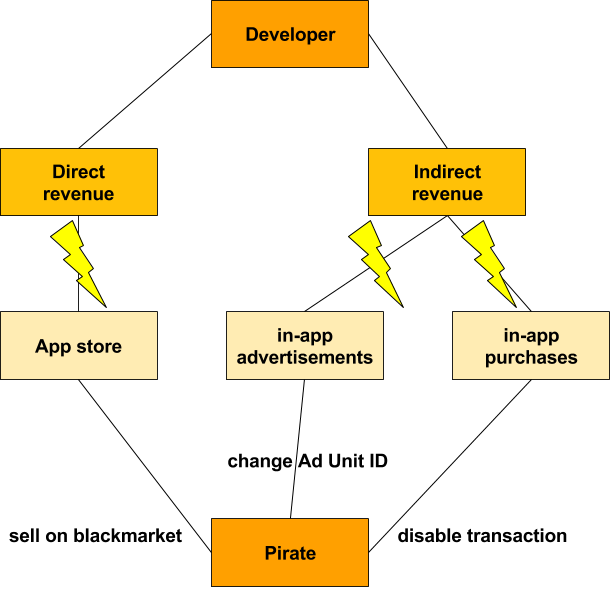
\includegraphics[width=0.8\textwidth]{data/revenue.png}
    \caption{Different ways to generate revenue}
    \label{fig:revenue}
\end{figure}
Beside monetary issues, additional problems arise when the application is moved to a black market store or website and distributed without the environment of an official app store.
The results is the loss of control over the application for the developer.
He can no longer provide support and updates for the application.
The users will not get fixes for security issues and crashes caused by malfunctions.
Users which do not know that they are using a pirated version will connect the unsatisfying behaviour to the developer.
This results in the loss of future revenues which are not even connected to this application.
\newline
The developer can face also unpredictable scenarios like unforseen traffic since the growth of the application cannot be monitored with tools provided by the marketplace of choice.
This can stress the server because they were not scaling accordingly.
As revenue from the application is stolen, there may not be enough money for upgrades necessary by legal and illegal use \cite{lierschDeveloperThreats}.
\newline
\newline
Developers make a living of their applications.
When they do not make a profit from their application, or even lose money with their servers, they can no longer continue.
The result is a loss of creativity, ideas and skill for the ecosystem.
